\documentclass[11pt]{article}
\usepackage[letterpaper,margin=1in]{geometry}
\usepackage[T1]{fontenc}
\usepackage{mathptmx}
\usepackage{amsmath,amssymb}
\usepackage{graphicx}
\usepackage{booktabs}
\usepackage[font=small,labelfont=bf]{caption}
\usepackage[numbers,sort&compress]{natbib}
\usepackage{xcolor}
\usepackage{microtype}
\usepackage{authblk}
\usepackage[colorlinks=true,linkcolor=blue!50!black,citecolor=blue!50!black,urlcolor=blue!50!black]{hyperref}
\setlength{\emergencystretch}{3em}
\renewcommand{\baselinestretch}{1.12}
\newcommand{\LIO}{\texorpdfstring{LaInO$_3$}{LaInO3}}
\newcommand{\BSO}{\texorpdfstring{BaSnO$_3$}{BaSnO3}}
\newcommand{\ns}{n_s}

\title{Intersubband optics of the polar \LIO/\BSO\ two-dimensional electron gas: fragmented hybrid plasmons, phonon-limited lifetimes, intrinsic second-order nonlinearity and the limits of electrolyte gating}
\author{Gracen Ownby}
\affil{University of Oklahoma, Norman, Oklahoma, USA}
\date{\small 13 October 2026}

\begin{document}
\maketitle

\begin{abstract}
The polar interface between \LIO\ and \BSO\ hosts a two-dimensional electron gas (2DEG) whose density has been raised to about $10^{14}$~cm$^{-2}$ by electric-double-layer gating, with low-temperature mobilities above 2000~cm$^2$/Vs. We know of no study of its optical response. We compute the intersubband (ISB) response of this 2DEG for sheet densities of $5\times10^{12}$--$1.2\times10^{14}$~cm$^{-2}$, for a strongly compensated ($N_A=5\times10^{19}$~cm$^{-3}$ acceptors) and a clean ($10^{18}$~cm$^{-3}$) \BSO\ layer. The model is a self-consistent Kane-nonparabolic Schr\"odinger--Poisson solution of the interface, with in-plane masses from the energy-dependent Hamiltonian and Fermi-level pinning by the acceptors, and a $k$-resolved random-phase (time-dependent Hartree) response that keeps in-plane nonparabolicity, the polar-phonon background and second-order terms.

The electrons sit at mean distances of 0.5--1.8~nm from the interface, with in-plane masses of 0.20--0.26~$m_0$. Below the density at which the \LIO\ cap starts to fill, the single-particle transition energy $E_{21}$ is 0.41--0.57~eV (compensated) and 0.13--0.44~eV (clean); local exchange and correlation would raise it by 6--59~meV, depending on how they are screened. Because the background permittivity at these energies is only about 4, Coulomb coupling raises the oscillator-strength-weighted mean absorption energy by factors of 1.07--1.62 (compensated) and 1.27--1.85 (clean) over the single-particle value. The bright $1\to2$ mode is pushed into the ladder of weak higher transitions and fragments: at $10^{14}$~cm$^{-2}$ the strongest mode carries 29\% (compensated) and 9\% (clean) of the absorption. Half of the absorption lies below 1.4--2.8~$\mu$m (compensated) and 1.5--5.4~$\mu$m (clean) in wavelength terms, depending on density.

With all positive charge at the interface the Fermi level reaches the \LIO\ conduction band near $1.1\times10^{14}$~cm$^{-2}$ (compensated). If the gate charge sits instead on the surface of a 5~nm \LIO\ cap, as in electrolyte gating, cap states start to fill after only $2.0$--$3.1\times10^{13}$~cm$^{-2}$ of added density, so that purely electrostatic gating through such a cap stays far below the reported $10^{14}$~cm$^{-2}$. With three polar LO modes (Fr\"ohlich constants summing to 1.3), the $2\to1$ lifetime of electrons excited from subband 1 is 32--79~fs. The asymmetric well has an intrinsic second-order susceptibility; for a 30~meV linewidth Coulomb screening reduces it by factors of 2--9, to 37--139~nm$^2$/V per interface. Over the literature ranges of seven material parameters, the acceptor density dominates the uncertainty of $E_{21}$, the collective absorption is about twice as robust, and at $10^{14}$~cm$^{-2}$ the Fermi level lies within 0.2~eV of the cap conduction band in 82\% of the parameter sets.
\end{abstract}

\section{Introduction}
\BSO\ is a wide-gap perovskite (indirect gap about 3.0~eV) with a dispersive Sn-5s conduction band and a band-edge mass of about 0.19~$m_0$ \cite{Niedermeier2017,Aggoune2022}. When \LIO\ is grown on it, the polar discontinuity between the neutral BaO/SnO$_2$ planes and the charged LaO$^+$/InO$_2^-$ planes creates a 2DEG on the \BSO\ side of the interface without intentional doping \cite{Kim2019LIO,Aggoune2021}. With an ionic liquid on a 5~nm \LIO\ cap, its density has been raised to about $10^{14}$~cm$^{-2}$ by electric-double-layer gating \cite{Lee2024LIO,Ueno2008}, with mobilities above 2000~cm$^2$/Vs at 10~K. The conduction-band offset is about 1.6~eV \cite{Kim2019LIO,Lee2024LIO}, and first-principles calculations place the 2DEG within 1--2~nm of the interface with a mass of 0.24~$m_0$ \cite{Aggoune2021}. All of this work concerns transport.

A strongly confined, dense 2DEG with a light mass and a large band offset is also an intersubband (ISB) system, and an unusual one. Its background permittivity at near-infrared frequencies is about 4, against 10--13 in III--V wells, so Coulomb effects on the ISB response are large. It is polar, so its ISB transitions couple strongly to LO phonons. And its confining potential is asymmetric by construction, so it has a second-order nonlinearity without compositional engineering. Oxide ISB optics is a young field: room-temperature ISB absorption has been measured in SrTiO$_3$/LaAlO$_3$ wells \cite{Ortmann2018}, and \BSO\ quantum wells with BaO, MgO or Al$_2$O$_3$ barriers have been modelled \cite{Li2021BSO,Stanojevic2023,Jang2023}. These studies treat doped, composition-defined wells with a phenomenological linewidth; the largest second-order susceptibility predicted is 200~nm/V under bias \cite{Li2021BSO}. A comparable treatment exists for $\beta$-Ga$_2$O$_3$ wells \cite{Lyman2020}. We know of no treatment of the polar \LIO/\BSO\ 2DEG, of the depolarization shift in a \BSO\ system, or of its ISB phonon lifetimes.

This paper computes the ISB response of the interface as a function of the sheet density. The results are: (i) the subband structure, how strongly the compensating acceptors in the \BSO\ set the confinement, and the densities at which the \LIO\ cap starts to fill, for a field-free cap and for electrolyte gating (Sec.~\ref{sec:sub}); (ii) the collective ISB response with in-plane nonparabolicity, which is shifted far above the single-particle transitions, splits among hybrid modes and moves from the mid- to the near-infrared with density (Sec.~\ref{sec:lin}); (iii) LO-phonon lifetimes with all three polar modes, Pauli blocking and screening (Sec.~\ref{sec:tau}); (iv) the intrinsic second-order susceptibility (Sec.~\ref{sec:chi2}); and (v) a Monte Carlo propagation of the uncertainty in the material parameters (Sec.~\ref{sec:uq}). Appendix~\ref{app:checks} collects the numerical and model checks. The calculations use qwkit \cite{qwkit}, extended for this work with a single-interface solver and a $k$-resolved collective response.

\section{Model}\label{sec:model}
\subsection{Material parameters}
Table~\ref{tab:par} lists the parameters and their ranges, from the sources compiled for this work. The \BSO\ band-edge mass and Kane nonparabolicity come from infrared measurements over $1.6\times10^{19}$--$7.3\times10^{20}$~cm$^{-3}$, which give $m^*=0.19\,m_0$ and $\beta=0.56$~eV$^{-1}$ in $E(1+\beta E)=\hslash^2k^2/2m^*$ \cite{Niedermeier2017}; first-principles calculations give 0.20~$m_0$ and $\beta=0.25$~eV$^{-1}$ \cite{Krishnaswamy2017}. These data constrain the dispersion up to kinetic energies of about 1~eV; the model uses it beyond that for the upper subbands (Sec.~\ref{sec:disc}). The three polar modes of \BSO\ are taken from infrared ellipsometry \cite{Stanislavchuk2012}. Reported values of the electronic permittivity $\varepsilon_\infty$ range from 3.3 (the high-frequency limit of the infrared fit) to 4.2--4.3 (near-infrared ellipsometry and first-principles calculations) \cite{Stanislavchuk2012,Krishnaswamy2017,Aggoune2022}; we use 4.0 and propagate 3.3--4.3 in Sec.~\ref{sec:uq}. With $\varepsilon_\infty=4.0$ the factorized dielectric function gives a static permittivity $\varepsilon_s=20.5$ (Lyddane--Sachs--Teller), consistent with the value of 20 used for Poisson's equation. The \LIO\ phonons are not known, so the cap is treated as a passive barrier. Kim \emph{et al.} found deep acceptors of $4$--$6\times10^{19}$~cm$^{-3}$ in their \BSO\ films \cite{Kim2019LIO}; we use $5\times10^{19}$~cm$^{-3}$ for the \emph{compensated} case and $10^{18}$~cm$^{-3}$ for a \emph{clean} film, and pin the Fermi level 1.0~eV below the bulk conduction band (0.5--1.5~eV in Sec.~\ref{sec:uq}).

\begin{table}[t]
\centering\small
\caption{Parameters (baseline and the range used in Sec.~\ref{sec:uq}).}\label{tab:par}
\begin{tabular}{lll}
\toprule
Quantity & Baseline & Range, source \\
\midrule
\BSO\ band-edge mass $m^*$ & 0.19~$m_0$ & 0.17--0.22 \cite{Niedermeier2017,Krishnaswamy2017,Aggoune2022} \\
\BSO\ nonparabolicity $\beta$ & 0.56~eV$^{-1}$ & 0.25--0.56 \cite{Niedermeier2017,Krishnaswamy2017} \\
\BSO\ $\varepsilon_\infty$ (ISB energies) & 4.0 & 3.3--4.3 \cite{Stanislavchuk2012,Krishnaswamy2017,Aggoune2022} \\
\BSO\ $\varepsilon_s$ (Poisson) & 20 & from $\varepsilon_\infty$ (LST): 16.9--22.0 \cite{Stanislavchuk2012} \\
\BSO\ TO/LO (cm$^{-1}$) & 135/154, 244.5/421, 628/723 & \cite{Stanislavchuk2012} \\
\LIO/\BSO\ conduction-band offset & 1.6~eV & 1.35--1.70 \cite{Kim2019LIO,Lee2024LIO,Aggoune2021} \\
\LIO\ band-edge mass & 0.46~$m_0$ & 0.30--0.50 \cite{Kim2019LIO,Aggoune2021,Jang2017LIO} \\
\LIO\ $\varepsilon_s$; Kane gap parameter & 24; 5~eV & fixed (assumed gap parameter) \\
\LIO\ cap thickness & 5~nm & 2--8~nm in checks \cite{Lee2024LIO} \\
Acceptors in \BSO\ $N_A$ & $5\times10^{19}$, $10^{18}$~cm$^{-3}$ & $10^{18}$--$5\times10^{19}$ (log) \cite{Kim2019LIO} \\
Pinning $E_c-E_F$ in bulk \BSO & 1.0~eV & 0.5--1.5 (assumed) \\
ISB linewidth $\gamma$ (half width) & 10~meV & 30~meV (room temperature) \\
\bottomrule
\end{tabular}
\end{table}

\subsection{Self-consistent interface}
The \LIO\ cap ($-d<z<0$, $d=5$~nm, closed by a hard wall that stands for the electrolyte) and the \BSO\ ($0<z<L$) are described by a one-band Kane Schr\"odinger equation with an energy-dependent mass $m(z,E)=m^*(z)[1+(E-V(z))\beta(z)]$ \cite{Nelson1987}, $H(E,k)=-\partial_z\frac{\hslash^2}{2m(z,E)}\partial_z+V(z)+\frac{\hslash^2k^2}{2m(z,E)}$. The in-plane band-edge mass of subband $n$ follows from first-order perturbation theory in $k^2$ with the energy dependence of $H$ \cite{Ekenberg1989},
\begin{equation}
\frac{1}{m_n}=\frac{\langle m(z,E_n)^{-1}\rangle_n}{1-\langle\partial_EH\rangle_n},\qquad \langle\partial_EH\rangle_n=-\frac{\hslash^2}{2}\int\frac{m^*\beta}{m(z,E_n)^2}\,|\psi_n'|^2\,dz,\label{eq:mass}
\end{equation}
which reduces to the bulk Kane result $m^*(1+2\beta T)$ for a flat well with kinetic energy $T$. The in-plane dispersion is written as
\begin{equation}
\frac{\hslash^2k^2}{2m_n}=\epsilon\left(1+\frac{\epsilon}{G_n}\right),\label{eq:disp}
\end{equation}
with $G_n$ fitted to the exact dispersion $E_n(k)$ of $H(E,k)$ over the occupied range (it reproduces $E_n(k)$ to 2\%); the subband density of states is then $(m_n/\pi\hslash^2)(1+2\epsilon/G_n)$, with Fermi--Dirac occupations.

The Hartree potential is generated by the electrons, by ionized acceptors over a depletion width $w_d$, and by a positive sheet charge $\sigma_+=n_s+N_\mathrm{dep}$ (polarization and gate charge, $N_\mathrm{dep}=N_Aw_d$) that neutralizes them. The depletion width follows from Fermi-level pinning in the bulk \BSO, $V(L)-E_F=E_\mathrm{pin}$. Where the positive charge sits matters for the cap. In the baseline all of it sits at the interface, so that the cap is field-free; this describes a density set at the interface itself (by the polarization charge, interface doping or a gate behind the 2DEG) and assumes that the bound charge of the polar \LIO\ is compensated at the cap surface. In electrolyte gating the gate charge sits on the cap surface instead; Sec.~\ref{sec:sub} treats this case with a fixed interface sheet. A local exchange-correlation potential (Hedin--Lundqvist \cite{HedinLundqvist1971}) is used as a check. The equations are discretized on a cell-centred grid (0.5~\AA\ in the compensated case, 1~\AA\ in the clean case) and solved with Anderson mixing, first with an approximate nonparabolicity and then with the fitted $G_n$ held fixed; the box length is $L=1.4\,w_d^{0}+15$~nm, clipped to 30--250~nm, where $w_d^0$ is the depletion width of the pinning voltage alone.

\subsection{\texorpdfstring{$k$}{k}-resolved collective response}
The subband wavefunctions at $k=0$ are kept, and each in-plane wavevector shell carries the occupations $f_n(k)$ and energies $E_n(k)$ of Eq.~\eqref{eq:disp}. The shells are coupled only through the Hartree potential of the total induced density. For a $z$-polarized drive, given as the field $E_d=D/\varepsilon_b$ the stack would have without the electrons,
\begin{align}
(\hslash\omega-E_{ab}(k)+i\gamma)\,\rho^{(1)}_{ab}(k)&=[f_b(k)-f_a(k)]\,\tilde U_{ab},\qquad \tilde U=eE_dz+U_H[X^{(1)}],\quad X^{(1)}=\sum_k w_k\rho^{(1)}(k),\\
U_H[X]_{ab}&=\frac{e^2}{\varepsilon_0\varepsilon_b(\omega)}\sum_{cd}S_{abcd}X_{cd},\qquad S_{abcd}=\int F_{ab}F_{cd}\,dz,\quad F_{ab}(z)=\int_{-\infty}^z\psi_a\psi_b\,dz',
\end{align}
where $\varepsilon_0$ is the vacuum permittivity, $w_k$ the sheet density of a shell ($k\,dk/\pi$, spin included) and $E_{ab}=E_a-E_b$. Both orderings of each pair are kept, so the response contains the antiresonant terms. The induced sheet dipole is $p=-e\sum_{ab}z_{ba}X_{ab}$, and the absorbed power per unit area is $(\omega/2)\,\mathrm{Im}\,p\,|E_d|^2$; for a thin layer this is the loss function measured in Brewster-angle or attenuated-total-reflection geometries. At second order,
\begin{align}
(2\hslash\omega-E_{ab}(k)+i\gamma)\,\rho^{(2)}_{ab}(k)&=[\tilde U,\rho^{(1)}(k)]_{ab}+[f_b(k)-f_a(k)]\,U_H[X^{(2)}]_{ab}\quad(a\neq b),\\
(2\hslash\omega+i\hslash/\tau_p)\,\rho^{(2)}_{aa}(k)&=[\tilde U,\rho^{(1)}(k)]_{aa},
\end{align}
with $U_H$ evaluated with $\varepsilon_b(2\omega)$, $X^{(2)}=\sum_kw_k\rho^{(2)}(k)$ and $\chi^{(2)}_s=-e\sum_{ab}z_{ba}X^{(2)}_{ab}/\varepsilon_0E_d^2$. The population time $\tau_p$ enters only the diagonal terms at $2\omega$, where it is irrelevant ($2\hslash\omega\gg\hslash/\tau_p$ for any $\tau_p$ above a few fs; we use 1~ps). The background permittivity $\varepsilon_b(\omega)=\varepsilon_\infty\prod_j(\omega_{Lj}^2-\omega^2-i\omega g)/(\omega_{Tj}^2-\omega^2-i\omega g)$ contains the three polar modes ($\hslash g=2$~meV); it is used throughout the stack, including the thin cap. With a single shell and no dispersion the equations reduce exactly to the subband-level time-dependent Hartree response \cite{AllenTsuiVinter1976,Ando1977,AndoRMP1982} already in qwkit; with the Hartree term off they give the single-particle response. Pairs of subbands that are both empty carry no first-order coherence and are dropped from the linear system (occupation differences below $10^{-5}$). All subbands up to 3~eV above $E_1$ are used, at most 90, which reach 2.1--2.6~eV in the clean case, with 200 shells (150 for $\chi^{(2)}$). Because the subbands are eigenstates of different energy-dependent Hamiltonians, their envelopes overlap slightly; they are orthonormalized by the symmetric (L\"owdin) procedure \cite{Lowdin1950} as a set that extends 0.6~eV beyond the kept range (12 states beyond it where the limit of 90 subbands is reached), so that the truncation does not distort the highest kept states. Appendix~\ref{app:checks} compares this with the two-band Kane states, which are orthogonal without this step.

\subsection{LO phonons}
Each polar mode $j$ couples with the Fr\"ohlich factor $C_j=(1/\varepsilon_\infty-1/\varepsilon_s)_j$ obtained from the residue of $1/\varepsilon_b(\omega)$ at its LO pole; the $C_j$ sum to $1/\varepsilon_\infty-1/\varepsilon_s$ \cite{Varga1965}. The corresponding Fr\"ohlich constants for $m^*=0.19\,m_0$ are 0.12, 0.76 and 0.45 for the 19, 52 and 90~meV modes (sum 1.32); with $\varepsilon_\infty=3.3$ and slightly different LO frequencies, Niedermeier \emph{et al.} obtained a sum of 1.5 \cite{NiedermeierPolaronArxiv}. The rate out of an electron of wavevector $k$ in subband 2 into subband 1 is the bulk-phonon rate \cite{Ridley1982} generalized to $k\neq0$: an angular integral over the final wavevector of $I_{21}(Q)/Q$, with $I_{21}$ the Coulomb form factor of the transition density $\psi_1\psi_2$ and $Q=|\mathbf k-\mathbf k'|$, the nonparabolic final density of states of Eq.~\eqref{eq:disp}, the phonon occupation, and Pauli blocking $1-f_1(k')$. It is averaged over the electrons that a vertical $1\to2$ excitation creates, with weight $f_1(k)[1-f_2(k)]$. Screening by the 2DEG is static RPA screening of the $2\to1$ vertex by the intrasubband polarization of the occupied subbands, with the two-dimensional Lindhard function, the form factors of the intersubband and intrasubband densities, and the background $\varepsilon_\infty$.

\subsection{Spectral measures}\label{sec:measures}
The centroid of a computed absorption spectrum is a poor measure of where the absorption lies: a Lorentzian line weighted by $\omega$ has a first moment that grows logarithmically with the upper end of the window, so that for a single line at 0.134~eV with $\gamma=10$~meV the centroid over 0.10--2.5~eV lies 25\% above the line. We use two other measures. The \emph{mean absorption energy} $\bar E$ is the oscillator-strength-weighted mean of the mode energies of the $k=0$ response, obtained exactly from the eigenvalue problem of the time-dependent Hartree equations \cite{AllenTsuiVinter1976,AndoRMP1982}, $\Omega^2=\mathsf E^2+2(\mathsf{EN})^{1/2}\mathsf K(\mathsf{EN})^{1/2}$, over all subband pairs $i$ with an occupation difference ($\mathsf E$ and $\mathsf N$ diagonal with the pair energies and sheet-density differences, $\mathsf K_{ij}=eS_{ij}/\varepsilon_0\varepsilon_\infty$). It is the first moment of the absorbed power, free of any linewidth; the collective oscillator strengths add up to the single-particle sum to $10^{-4}$ (for nonparabolic subbands that sum differs from the parabolic value \cite{Sirtori1994}). The ratio of $\bar E$ to the single-particle mean $\sum_if_iE_i/\sum_if_i$, the \emph{collective blue-shift factor}, measures the Coulomb shift. The $k=0$ problem omits the in-plane spread and the phonon background, both small corrections here (Appendix~\ref{app:checks}). For the $k$-resolved spectra we give the \emph{median} (the photon energy below which half the power in 0.10--2.5~eV is absorbed; 2.5\% above a single line at 0.134~eV for $\gamma=10$~meV, 17\% for 30~meV, and less than 0.5\% above lines at 0.3~eV or higher for 10~meV), the strongest peak, and the fraction $f_{50}$ of the absorption within $\pm50$~meV of that peak, which is 0.88 for a single Lorentzian line with $\gamma=10$~meV and 0.66 for 30~meV. In a spectrum with several modes the median can fall between peaks.

\section{Subband structure and the gating limit}\label{sec:sub}
Figure~\ref{fig:sub}a shows the self-consistent potential at $3\times10^{13}$ and $10^{14}$~cm$^{-2}$ in the compensated case. The well is triangular near the interface. The depletion charge of the acceptors, $4.1$--$4.7\times10^{13}$~cm$^{-2}$ over 8.2--9.3~nm, is comparable to the 2DEG and steepens the well. The mean distance of the ground subband from the interface falls from 8.1 to 4.9~\AA\ as the density rises from $5\times10^{12}$ to $1.2\times10^{14}$~cm$^{-2}$; in the clean case (depletion charge $5.1$--$5.4\times10^{12}$~cm$^{-2}$ over 51--54~nm) it falls from 18.1 to 6.2~\AA. The in-plane band-edge mass of the ground subband, Eq.~\eqref{eq:mass}, is 0.230--0.255~$m_0$ and 0.203--0.240~$m_0$ in the two cases, close to the 0.24~$m_0$ of first-principles calculations \cite{Aggoune2021}, and the 2DEG lies within the 1--2~nm found there. A mean distance of 5--8~\AA\ is 1.2--2 \BSO\ unit cells. The envelope-function approximation is then at its limit: Li \emph{et al.} found effective-mass and Wannier tight-binding levels in agreement for \BSO\ wells of 3--7 unit cells \cite{Li2021BSO}, which does not cover the densest cases here. The predictions at the highest densities are therefore indicative.

\begin{figure}[t]
\centering
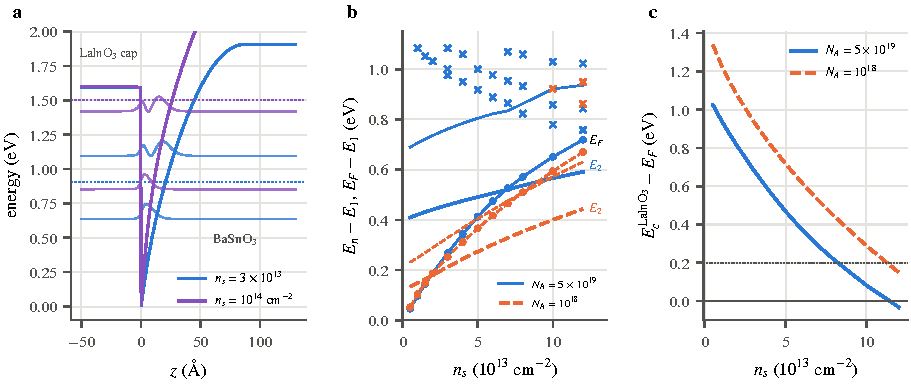
\includegraphics[width=\textwidth]{figures/fig1_subbands.pdf}
\caption{(a) Self-consistent conduction band, first two subbands (squared wavefunctions offset by their energies) and Fermi level (dotted) at $\ns=3\times10^{13}$ and $10^{14}$~cm$^{-2}$, compensated case, 300~K, including the 5~nm \LIO\ cap; energies from the conduction band at the interface. (b) $E_2-E_1$ (thick), $E_3-E_1$ of the third \BSO\ subband (thin) and $E_F-E_1$ (dots) against density, compensated (solid) and clean (dashed); crosses mark states with more than half their weight in the \LIO\ cap. (c) Distance of the Fermi level below the lowest conduction-band energy of the \LIO\ cap, with all positive charge at the interface.}
\label{fig:sub}
\end{figure}

The single-particle transition energy $E_{21}$ is 0.41--0.59~eV in the compensated case and 0.13--0.44~eV in the clean case over $5\times10^{12}$--$1.2\times10^{14}$~cm$^{-2}$ (Fig.~\ref{fig:sub}b): the compensation of the bulk \BSO\ shifts it by up to 0.28~eV at equal density. The second subband starts to fill at 5--$6\times10^{13}$~cm$^{-2}$ in the compensated case. In the clean case it holds 2--4\% of the electrons at 300~K below $10^{13}$~cm$^{-2}$ (thermally; at 10~K it is empty there) and about a fifth from $5\times10^{13}$~cm$^{-2}$ on.

\emph{Field-free cap.} With all positive charge at the interface the Fermi level rises by 0.67~eV above $E_1$ over the density range. It comes within 0.2~eV of the lowest conduction-band energy of the cap at $8.2\times10^{13}$~cm$^{-2}$ and reaches it at about $1.14\times10^{14}$~cm$^{-2}$ in the compensated case (Fig.~\ref{fig:sub}c); in the clean case the margin is still 0.15~eV at $1.2\times10^{14}$~cm$^{-2}$. Beyond that point the states of the cap fill and conduction becomes parallel. The cap, closed by a hard wall, has its own quantized states. In the compensated case the lowest of them, which descends from about 1.05~eV above $E_1$ at $1.5\times10^{13}$~cm$^{-2}$ to 0.76~eV at $1.2\times10^{14}$~cm$^{-2}$, becomes the third state of the system from $8\times10^{13}$~cm$^{-2}$ on (crosses in Fig.~\ref{fig:sub}b); at $1.2\times10^{14}$~cm$^{-2}$ it holds about 1\% of the electrons.

\emph{Electrolyte gating.} An ionic liquid places the gate charge on the cap surface, and the field it creates across the cap lowers the cap conduction band towards the surface. To model this we fix the positive sheet at the interface at the value that gives an ungated density $n_0$ ($5\times10^{12}$, $10^{13}$ or $2\times10^{13}$~cm$^{-2}$; the ungated density of the gated samples was not reported \cite{Lee2024LIO}) and put the remaining positive charge on the cap surface. The Fermi level reaches the cap conduction-band edge at the surface after an added density of $1.6$--$1.9\times10^{13}$~cm$^{-2}$ in the compensated case and $2.2$--$2.5\times10^{13}$~cm$^{-2}$ in the clean case (5~nm cap, $\varepsilon_s=24$). Because the lowest accumulation state at the surface lies above that edge, filling starts somewhat later: cap-localized states hold 1\% of the electrons after an added density of $2.0$--$2.3\times10^{13}$ and $2.6$--$3.1\times10^{13}$~cm$^{-2}$, that is, at $n_s=2.8$--$4.0\times10^{13}$ and $3.6$--$4.6\times10^{13}$~cm$^{-2}$. A cap permittivity of 50 raises the added density at this point to $3.2$--$3.8\times10^{13}$ and $4.2$--$5.1\times10^{13}$~cm$^{-2}$, and a 2~nm cap to $5.1$--$5.6\times10^{13}$ and $6.2$--$7.2\times10^{13}$~cm$^{-2}$. The order of magnitude follows from a capacitor estimate: a cap of thickness $d$ holds $\varepsilon_0\varepsilon_s/(e^2d)\approx2.7\times10^{13}$~cm$^{-2}$ per eV of margin between the Fermi level and the cap band; the computed values lie below this because the margin also shrinks as the Fermi level rises with density. Purely electrostatic accumulation at the buried interface through a 5~nm \LIO\ cap therefore stops below $5\times10^{13}$~cm$^{-2}$ in this model, well below the $10^{14}$~cm$^{-2}$ reported with an ionic liquid on such a cap \cite{Lee2024LIO}. Either the cap screens better than its static permittivity suggests at these fields, or the offset is larger, or part of the measured charge resides at or near the cap surface, or the gating is partly electrochemical (Sec.~\ref{sec:disc}). In what follows the density is treated as a parameter with the field-free cap; Appendix~\ref{app:checks} shows how the spectra change when part of the positive charge sits on the cap surface.

\section{Collective intersubband response}\label{sec:lin}
Figure~\ref{fig:spec} maps the absorbed power against photon energy and density. The single-particle spectra (a, b) follow $E_{21}$, red-shifted by in-plane nonparabolicity: across the Fermi sea the $1\to2$ energy changes by about $(1-m_1/m_2)(E_F-E_1)$. In the compensated case $m_2$ exceeds $m_1$ by 8--10\%, and the single-particle line widens from 15 to 75~meV (full width on the 5~meV grid, which underestimates it by up to one grid step), against 20~meV for the homogeneous width; its median lies up to 9\% below $E_{21}$. In the clean case the two masses differ by less than 3.3\% and the line stays narrow. In the compensated case the $1\to3$ and higher transitions are weak ($z_{13}\le1.25$~\AA\ against $z_{12}=4.3$--5.4~\AA), and the $1\to2$ transition carries 86--87\% of the $1\to n$ oscillator strength; in the clean case the dense ladder of states on the shallow depletion slope gives several transitions of comparable strength, and $1\to2$ carries 65--76\%. The single-particle mean absorption energy therefore lies 4--20\% above $E_{21}$ in the compensated case (up to $10^{14}$~cm$^{-2}$) and up to 48\% above it in the clean case.

\begin{figure}[t]
\centering
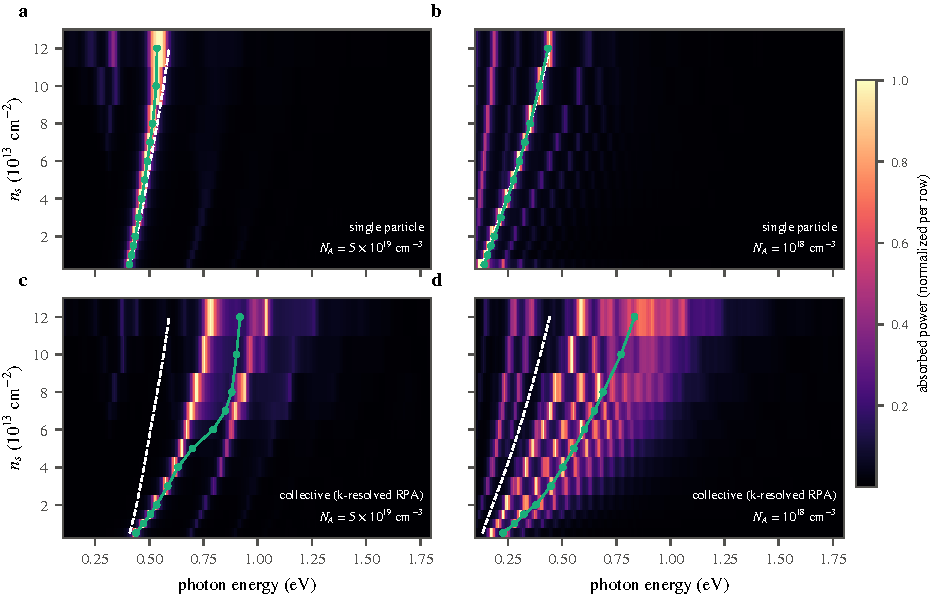
\includegraphics[width=\textwidth]{figures/fig2_spectra.pdf}
\caption{Absorbed power against photon energy for single-particle (a, b) and collective (c, d) response, compensated (a, c) and clean (b, d) case, 300~K, $\gamma=10$~meV. Each row is normalized to its maximum above 0.15~eV and the colour scale is clipped at 1 (in the clean case at $5\times10^{12}$ and $10^{13}$~cm$^{-2}$, where the single-particle peak lies below 0.15~eV, the rows saturate). White dashed lines: $E_{21}$. Green dots: median of the absorption over 0.10--2.5~eV.}
\label{fig:spec}
\end{figure}

The collective response (c, d) is shifted far to the blue. Its mean absorption energy rises from 0.52 to 0.95~eV in the compensated case (up to $10^{14}$~cm$^{-2}$, below the filling of the cap) and from 0.25 to 0.81~eV in the clean case (Fig.~\ref{fig:coll}a). The collective blue-shift factor is 1.07--1.62 and 1.27--1.85 in the two cases and grows with density; relative to $E_{21}$ the mean lies 1.3--1.7 and 1.8--2.2 times higher. The $1\to2$ transition dressed alone, $E_{21}(1+\alpha)^{1/2}$ with the depolarization factor $\alpha$ \cite{AllenTsuiVinter1976,Ando1977}, would lie at 0.44--0.86 and 0.18--0.67~eV; the rest of the shift comes from its coupling to the higher transitions. The shift is large because the density is 10--240 times that of the III--V reference well of Sec.~\ref{sec:chi2} while the background permittivity, about 4, is a third of the III--V value. Half of the collective absorption lies below 0.44--0.90~eV (compensated, up to $10^{14}$~cm$^{-2}$) and 0.23--0.83~eV (clean), that is, the median wavelength is 1.37--2.83 and 1.49--5.45~$\mu$m; the strongest peaks lie at 1.64--2.85 and 1.85--7.1~$\mu$m. Within the densities that electrolyte gating reaches in our model (Sec.~\ref{sec:sub}), the median wavelength covers 2.0--2.8 and 2.3--5.4~$\mu$m.

\begin{figure}[t]
\centering
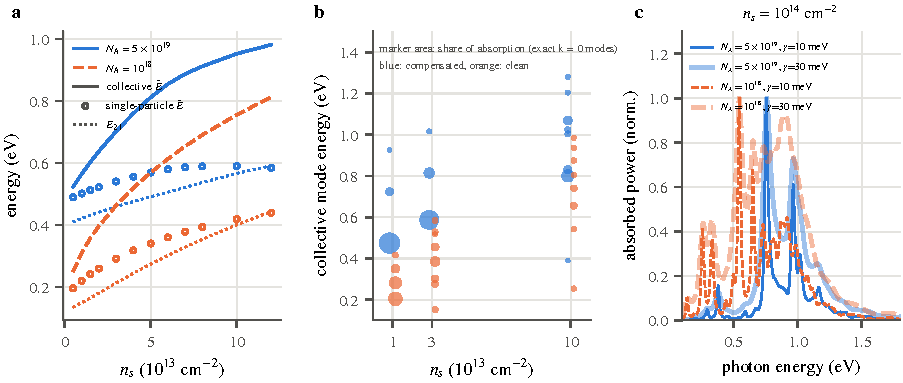
\includegraphics[width=\textwidth]{figures/fig3_collective.pdf}
\caption{(a) Mean absorption energy $\bar E$ of the collective (lines) and single-particle (open symbols) response, from the exact $k=0$ modes, and $E_{21}$ (dotted), compensated (blue, solid) and clean (orange, dashed). (b) Collective modes of the exact $k=0$ response at three densities; marker area is the share of the absorption carried by each mode (modes carrying more than 3\% shown; blue compensated, orange clean). (c) Collective $k$-resolved spectra at $10^{14}$~cm$^{-2}$ for $\gamma=10$~meV (thin) and 30~meV (thick, translucent), each normalized to its maximum.}
\label{fig:coll}
\end{figure}

The collective oscillator strength does not stay in one mode. In heavily doped III--V wells with many occupied subbands, the Coulomb coupling concentrates the strength of many transitions of similar dipole into one multisubband plasmon once the plasma energy exceeds the spread of the transition energies \cite{Delteil2012,Vasanelli2020}. Here the strength is dominated by one transition, $1\to2$, and the depolarization shift that pushes it up grows with density until it is comparable to the spacing of the weak transitions above it: in the compensated case the dressed $1\to2$ energy lies 0.03~eV above $E_{21}$ at $5\times10^{12}$~cm$^{-2}$ and 0.30~eV above it at $10^{14}$~cm$^{-2}$, while $E_{31}$ lies 0.2--0.3~eV above $E_{21}$; once the second subband fills, the $2\to n$ transitions join the ladder. The coupling matrix $\mathsf K$ is not dominated by one eigenvector (its largest eigenvalue carries 53--74\% of the trace of the coupling term). The bright mode therefore anticrosses with the ladder and fragments rather than condensing. The exact $k=0$ modes show this (Fig.~\ref{fig:coll}b). In the compensated case the strongest mode carries 79\% of the absorption at $10^{13}$~cm$^{-2}$ and 68\% at $3\times10^{13}$~cm$^{-2}$, but 29\% at $10^{14}$~cm$^{-2}$. In the clean case it carries 45\% at $5\times10^{12}$~cm$^{-2}$, 35\% at $10^{13}$~cm$^{-2}$ and 9\% at $10^{14}$~cm$^{-2}$. Correspondingly, in the $k$-resolved spectra $f_{50}$ falls from 0.72 to 0.29 (compensated, up to $10^{14}$~cm$^{-2}$) and from 0.47 to 0.12 (clean) as the density rises, against 0.88 for a single line, while for the single-particle spectra it falls only from 0.74 to 0.62 and from 0.66 to 0.37. With $\gamma=30$~meV, $f_{50}$ is 0.23--0.53 and 0.12--0.40 over the same density ranges (0.66 for a single line; Fig.~\ref{fig:coll}c), and the medians move up by at most 9\%.

From $8\times10^{13}$~cm$^{-2}$ on, the modes of the compensated case lie at the energies of the quantized cap states (0.78--0.86~eV above $E_1$ at $10^{14}$~cm$^{-2}$), whose positions depend on the cap thickness and on the hard wall that closes it. With caps of 3, 5 and 8~nm the median at $10^{14}$~cm$^{-2}$ changes by less than 0.7\% and $f_{50}$ stays at 0.27--0.31, but the share of the strongest peak in the $\gamma=2$~meV spectrum with phonon background, the decomposition used for these checks, changes (19--25\%, against 25\% for the 5~nm cap). Removing the cap states from this energy range, by raising the offset to 3~eV, leaves the absorption fragmented (at $10^{14}$~cm$^{-2}$ the strongest peak then carries 29\% instead of 25\%, and $f_{50}=0.32$ instead of 0.29) but moves the median up by 6.5--11\% at 8--$10\times10^{13}$~cm$^{-2}$ (and by $-1$\% at $6\times10^{13}$~cm$^{-2}$): the fragmentation is intrinsic, while the position of the absorption at these densities depends on the cap states. In the clean case the medians at $3\times10^{13}$ and $10^{14}$~cm$^{-2}$ change by less than 0.5\% with the cap thickness and the share of the strongest mode by at most 0.03. The numerical checks of Appendix~\ref{app:checks} change the medians by less than 0.25\%; model variants change them by a few per cent (two-band Kane transition densities $-1.4$ to $-3.9$\%, the $k=0$ response up to 2.1\%), local exchange and correlation by 1--10\% depending on their screening, and positive charge on the cap surface by up to 27\% once the cap fills; at 10~K the collective medians differ from the 300~K values by at most 0.5\%, because the 2DEG is degenerate.

Two effects outside the model matter at the highest densities. The quasi-static loss function omits the radiative (superradiant) damping of the bright mode \cite{Vasanelli2020}; for a single sheet at $10^{14}$~cm$^{-2}$ with an oscillator strength near 1 we estimate it at several meV off normal incidence, comparable to $\gamma=10$~meV. And the single-pass absorption of such a sheet is no longer small, so that measured absorbance is not simply proportional to the loss function.

\section{LO-phonon lifetimes}\label{sec:tau}
\BSO\ couples strongly to its polar phonons. The 52 and 90~meV modes contribute 40--45\% and 51--57\% of the $2\to1$ rate, the 19~meV mode about 3\%. Figure~\ref{fig:life}a shows the lifetime of the electrons that a vertical $1\to2$ excitation places in subband 2, with Pauli blocking and static screening, and two simpler estimates. In the compensated case it is 34--53~fs, rising with density because $E_{21}$ moves away from the LO energies and the emission wavevector grows. In the clean case it is 32--79~fs, or 28~fs at $5\times10^{12}$~cm$^{-2}$ without screening, which is not static there (below). This corresponds to a lifetime contribution $\hslash/2\tau$ of 4--12~meV to the half-width. Reported values of $\varepsilon_\infty$ for \BSO\ range from 3.3 to 4.3 (Sec.~\ref{sec:model}); with 3.3 the Fr\"ohlich coupling is 21\% stronger and the lifetimes correspondingly shorter, a range that Sec.~\ref{sec:uq} propagates.

Averaging over the excited electrons shortens the lifetime by 16--18\% in the compensated case, because electrons at finite $k$ can emit at smaller wavevector transfer; in the clean case, where $E_{21}$ is close to the LO energies, it changes it by $-5$ to $+12$\%. Pauli blocking matters once the final states of LO emission, at $E_{21}-\hslash\omega_{LO}$ above $E_1$, fall below the Fermi level: in the compensated case from $5\times10^{13}$~cm$^{-2}$ on (up to 14\%), in the clean case at all densities (up to 58\%). Screening is weak in the compensated case and moderate in the clean case. The intersubband transition density $\psi_1\psi_2$ couples to the intrasubband polarization of the 2DEG only through the overlap of the form factors, so the static RPA factor at the emission wavevector is 0.89--0.97 (compensated) and 0.72--0.90 (clean), and screening lengthens the lifetime by 3--12\% and 14--34\%. Static screening needs $\hslash Qv_F\gg\hslash\omega_{LO}$, with $v_F$ the Fermi velocity of subband 1. The ratio is 2.7--22 in the compensated case, but only 1.1--2.5 in the clean case at the lowest densities, where dynamic screening, which is weaker, would leave the lifetime nearer the unscreened value. A two-dimensional Thomas--Fermi screen of the bare Fr\"ohlich vertex, which ignores the form factors, would overstate the screening badly.

The calculation describes electrons excited vertically from subband 1 into subband 2. Where the absorption is fragmented among hybrid modes, in the clean case and in the compensated case from about $5\times10^{13}$~cm$^{-2}$ on (Sec.~\ref{sec:lin}), a mode involves several transitions and its decay is not that of a single excited electron; the numbers are then indicative of the scattering rate rather than of a mode lifetime. The model also omits interface and cap phonons, the coupling of the 2DEG plasmon to the LO phonons at the highest densities, and polaron shifts, which are of order $\sum_j\alpha_j\hslash\omega_{LO,j}\approx80$~meV for each subband and largely cancel in $E_{21}$.

For comparison, the transport mobility of 2100~cm$^2$/Vs at 10~K corresponds to $\hslash/\tau_\mathrm{tr}\approx2.8$~meV for a mass of 0.2~$m_0$ (a half width of 1.4~meV) \cite{Lee2024LIO}. At room temperature, mobilities of about 80~cm$^2$/Vs have been compiled for the ungated interface \cite{Ngabonziza2024}, a half width of about 35~meV; the transport rate is then dominated by intrasubband LO scattering, which does not broaden the intersubband line in the same way. ISB linewidths are usually broader than the transport value at low temperature because interface roughness acts on the intersubband transition directly. At 300~K the LO contribution alone is 4--12~meV. We therefore take $\gamma=10$~meV for the spectra, where it resolves the mode structure and represents a high-quality or low-temperature case, and 30~meV as the room-temperature estimate.

\begin{figure}[t]
\centering
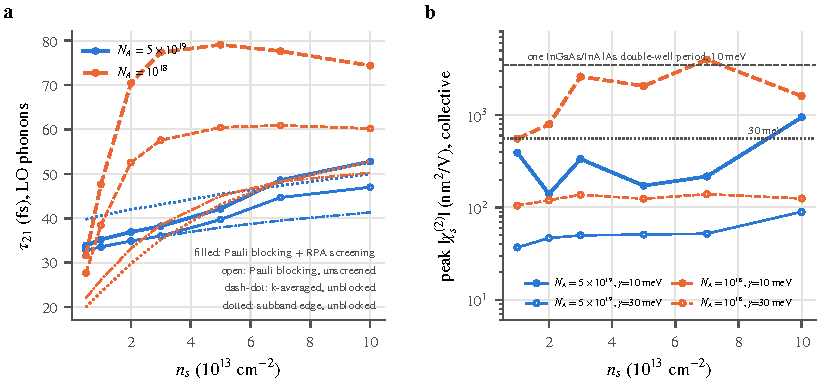
\includegraphics[width=\textwidth]{figures/fig4_lifetime_chi2.pdf}
\caption{(a) LO-phonon $2\to1$ lifetime of the electrons created by a vertical $1\to2$ excitation, with Pauli blocking and static RPA screening (filled), with Pauli blocking only (open), averaged over $k$ without either (dash-dot), and for an electron at the bottom of subband 2 without either (dotted), 300~K; compensated (blue) and clean (orange). (b) Peak sheet second-order susceptibility of the collective response over pump energies of 0.10--1.2~eV for $\gamma=10$~meV (filled) and 30~meV (open). Thin horizontal lines: one 21.4~nm period of the InGaAs/InAlAs asymmetric double well of Sec.~\ref{sec:chi2} at $5\times10^{11}$~cm$^{-2}$ for $\gamma=10$ (dashed) and 30~meV (dotted).}
\label{fig:life}
\end{figure}

\section{Second-order nonlinearity}\label{sec:chi2}
The triangular polar well breaks inversion symmetry, so $\chi^{(2)}_{zzz}$ is nonzero without compositional asymmetry, and its magnitude follows the density. For a single interface we report the sheet susceptibility for second-harmonic generation, $\chi^{(2)}_s=P^{(2)}_\mathrm{sheet}/\varepsilon_0E_d^2$, and take the peak of its modulus over pump energies of 0.10--1.2~eV (0.01~eV grid, refined to 1~meV around the three largest maxima), for $\gamma=10$ and 30~meV, at densities of $10^{13}$--$10^{14}$~cm$^{-2}$.

In the single-particle response of the compensated case the peak lies at $2\hslash\omega\approx E_{21}$ up to $7\times10^{13}$~cm$^{-2}$, where the two-level term $z_{12}^2(z_{22}-z_{11})$ of an asymmetric well dominates \cite{RosencherBois1991}; in the clean case, with its denser ladder of states, several resonances compete and the peak lies at pump energies of 0.10--0.14~eV. The peak is 180--470~nm$^2$/V ($\gamma=10$~meV) and 65--210~nm$^2$/V (30~meV) in the compensated case, and 2100--5000 and 660--1080~nm$^2$/V in the clean case, where the less confined states have longer dipoles ($z_{12}=9.0$ against 5.3~\AA\ at $10^{13}$~cm$^{-2}$). At the two lowest densities of the clean case the 30~meV peak lies at the lower end of the pump range, next to the 90~meV LO phonon, and is a lower bound.

The Coulomb coupling changes this picture. The depolarization field screens the drive below the collective resonances, at $\omega$ and at $2\omega$, and moves the resonances to the hybrid-mode energies of Sec.~\ref{sec:lin}. With $\gamma=30$~meV the collective peak is 37--90~nm$^2$/V in the compensated case and 105--139~nm$^2$/V in the clean case (Fig.~\ref{fig:life}b), 1.8--4.1 and 5.5--8.6 times below the single-particle values, at pump energies of 0.24--0.38 and 0.12--0.23~eV. The highest compensated value (90~nm$^2$/V, at $10^{14}$~cm$^{-2}$) involves the cap-state hybrids of Sec.~\ref{sec:lin}; at the densities that electrolyte gating reaches in our model the compensated values are 37--50~nm$^2$/V. With $\gamma=10$~meV the collective peaks, 140--940 and 560--4000~nm$^2$/V, vary irregularly with density, and at two densities of the compensated case they exceed the single-particle peaks. They occur where one hybrid mode lies at $\hslash\omega$ and another at $2\hslash\omega$: at $10^{13}$~cm$^{-2}$ in the compensated case, for example, the pump at 0.464~eV is resonant with the bright mode at 0.48~eV and its harmonic with the mode at 0.93~eV. Such coincidences depend on details of the mode spectrum that the model does not fix reliably, so only the 30~meV values should be read as predictions.

For comparison we designed, by a scan of layer widths, an InGaAs/InAlAs asymmetric double well for double resonance in the sense of Refs.~\cite{RosencherBois1991,Vurgaftman1996SSC}: 70/12/32~\AA\ with 100~\AA\ barriers and $5\times10^{11}$~cm$^{-2}$, with self-consistent $E_{21}=0.110$ and $E_{31}=0.217$~eV. We computed one period with the same collective equations for a single shell, a constant background permittivity of 10.9 and no phonons. For $\gamma=10$~meV its peak, 3490~nm$^2$/V ($1.6\times10^5$~pm/V over its 21.4~nm period), is doubly resonant at a pump energy of 0.110~eV; for 30~meV the double resonance is washed out and the peak, 555~nm$^2$/V, lies at $2\hslash\omega\approx E_{21}$. The comparison depends on which linewidths are realistic for each system. At the same $\gamma=30$~meV a \LIO/\BSO\ interface carries 0.07--0.16 (compensated) and 0.19--0.25 (clean) of the nonlinearity of one period. A half-width of 30~meV is pessimistic for an InGaAs well at 0.11~eV; against the 10~meV reference the ratios are 0.01--0.04. The lower refractive index of \BSO\ (about 2, against 3.3) favours it by a factor of about 4.5 in the usual conversion figure of merit $|\chi^{(2)}|^2/n^3$. The intrinsic nonlinearity of the polar well is thus modest; what it offers is a resonance at 3.3--10~$\mu$m pump wavelength, set by the density. Li \emph{et al.} predicted up to 200~nm/V for biased \BSO/BaO wells about 5~nm wide \cite{Li2021BSO}, about $10^{3}$~nm$^2$/V as a sheet value, from a single-particle model; our single-particle values are of the same order, and the collective reduction found here should apply to heavily doped oxide wells in general.

\section{Parameter uncertainty}\label{sec:uq}
We drew 100 Latin-hypercube samples of the seven material parameters of Table~\ref{tab:par} that carry a range (the acceptor density log-uniform, the others uniform; $\varepsilon_s$ follows from $\varepsilon_\infty$ by the Lyddane--Sachs--Teller relation) and repeated the calculations at $3\times10^{13}$ and $10^{14}$~cm$^{-2}$, 300~K; all samples converged. Figure~\ref{fig:uq} summarizes the results.

At $3\times10^{13}$~cm$^{-2}$ the 90\% intervals are 0.22--0.44~eV for $E_{21}$ and 0.46--0.66~eV for the median of the collective absorption; at $10^{14}$~cm$^{-2}$ they are 0.40--0.56 and 0.76--0.92~eV. The collective absorption is the more robust prediction: the relative 90\% width of its median is half that of $E_{21}$ (0.39 against 0.78, and 0.20 against 0.34). The collective blue-shift factor lies in 1.35--1.61 at $3\times10^{13}$~cm$^{-2}$ and 1.65--1.87 at $10^{14}$~cm$^{-2}$ in 90\% of the samples, so the large Coulomb shift does not depend on the parameter choice. The acceptor density dominates $E_{21}$ (Spearman rank correlation 0.90--0.96) and the collective median at $3\times10^{13}$~cm$^{-2}$ (0.85); at $10^{14}$~cm$^{-2}$ the median depends about equally on $\varepsilon_\infty$ ($-0.67$) and on the acceptor density ($+0.62$). The peak sheet susceptibility for $\gamma=30$~meV spans 48--133~nm$^2$/V at $3\times10^{13}$ and 68--190~nm$^2$/V at $10^{14}$~cm$^{-2}$. The LO-phonon lifetime spans 35--81 and 53--90~fs and is controlled by the acceptor density, $\varepsilon_\infty$ and the nonparabolicity. At $10^{14}$~cm$^{-2}$ the Fermi level lies within 0.2~eV of the lowest cap conduction-band energy in 82\% of the samples and above it in 20\%; the offset and the acceptor density decide which. At $3\times10^{13}$~cm$^{-2}$ the margin is about 0.5~eV or more in 95\% of the samples.

\begin{figure}[t]
\centering
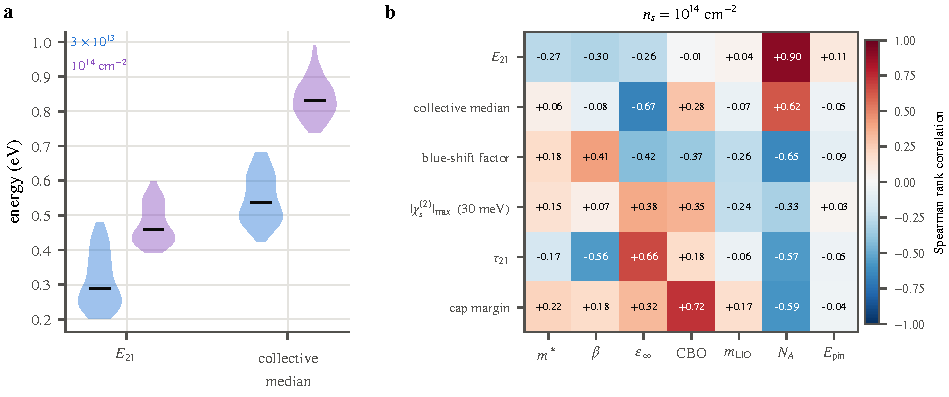
\includegraphics[width=\textwidth]{figures/fig5_uq.pdf}
\caption{Parameter uncertainty (100 Latin-hypercube samples over the ranges of Table~\ref{tab:par}, 300~K). (a) Distributions of $E_{21}$ and of the collective median at $3\times10^{13}$ and $10^{14}$~cm$^{-2}$ (bars: medians of the distributions). (b) Spearman rank correlation between each parameter and each prediction at $10^{14}$~cm$^{-2}$.}
\label{fig:uq}
\end{figure}

\section{Discussion}\label{sec:disc}
\emph{What the predictions rest on.} The largest single uncertainty is the compensation of the bulk \BSO, which sets the depletion field and therefore $E_{21}$, the subband occupations, the lifetimes and the nonlinearity (Sec.~\ref{sec:uq}). The collective absorption, which is what a measurement sees, depends on it less, and at the highest densities $\varepsilon_\infty$ matters as much. Since $E_{21}$ and the absorption energies depend about as strongly on the compensation as on the density, one ISB energy cannot fix both; the Hall density together with the median absorption energy, or the median together with $f_{50}$ as functions of gate voltage, could. Local exchange and correlation are a systematic uncertainty of the same order: screened by $\varepsilon_\infty$, which is arguably appropriate for electrons whose Fermi energy is far above the LO energies, they raise $E_{21}$ by 39--59~meV and the collective medians by 7--10\% (Appendix~\ref{app:checks}).

\emph{Collective physics.} With $\varepsilon_\infty\approx4$ and densities of $10^{13}$--$10^{14}$~cm$^{-2}$, the \LIO/\BSO\ 2DEG is far into the regime where the single-particle picture fails: the absorption would lie well above $E_{21}$ and split into several hybrid modes. Analyses of oxide ISB data that identify the absorption peak with a subband spacing would overestimate the confinement. The same physics limits the nonlinearity at realistic linewidths: the depolarization field that blue-shifts the absorption also screens the drive. Designs that rely on single-particle $\chi^{(2)}$ estimates for heavily doped oxide wells should be revisited with the collective response.

\emph{Gating.} Within this model, electrostatic gating through a 5~nm \LIO\ cap cannot reach the reported $10^{14}$~cm$^{-2}$ at the buried interface without the cap surface filling first: the cap acts as a capacitor that can hold about $\varepsilon_0\varepsilon_s/(e^2d)\approx2.7\times10^{13}$~cm$^{-2}$ per eV of the margin between the Fermi level and the cap band. The field-free baseline, in turn, assumes that the polarization charge of the \LIO\ is compensated at the cap surface; in the interface-polarization picture of Ref.~\cite{Kim2019LIO} the ungated cap need not be field-free. Whether the reported densities reflect better screening by the cap, a larger offset, charge near the cap surface or electrochemistry is an open question that combined transport and ISB measurements could answer.

\emph{Limitations.} The envelope-function approximation is at its limit for 0.5--1~nm confinement. The Kane dispersion of \BSO\ is constrained by experiment up to about 1~eV of kinetic energy, while the Fermi level lies up to 1.4--1.6~eV above the interface conduction band and the hybrid modes involve states up to 1.2~eV above $E_1$; the two-band check of Appendix~\ref{app:checks} tests the internal consistency of the one-band reduction, with a fictitious valence band at $1/\beta=1.8$~eV, not its validity at these energies. The \LIO\ phonons and interface phonon modes are unknown and are not included; nor are polaron corrections or radiative damping. Screening of the LO-phonon interaction is static. The response uses the \BSO\ background permittivity everywhere, including the thin cap. The cap is closed by a hard wall, which stands for the electrolyte, and its quantized states affect the mode decomposition at the highest densities of the compensated case. The ISB linewidth is a fixed parameter, and inhomogeneous gating would add to it. Exchange and correlation are treated only in the local approximation, as checks.

\section{Conclusion}
The \LIO/\BSO\ 2DEG is an intrinsically asymmetric, densely populated ISB system with a small background permittivity and strong polar coupling. Coulomb coupling raises its mean absorption energy by factors of 1.07--1.85 over the single-particle value and fragments the absorption among hybrid modes at high density; depending on density and compensation, half of the absorption lies below 1.4--5.4~$\mu$m. The LO-phonon lifetime of the excited electrons is 32--79~fs. A single interface carries a second-order susceptibility of 37--139~nm$^2$/V at a realistic room-temperature linewidth, reduced several-fold by the same Coulomb effects that shift the absorption. With a field-free cap the density can be raised to about $1.1\times10^{14}$~cm$^{-2}$ before the \LIO\ cap fills; with the gate charge on the cap surface, electrostatic gating through a 5~nm cap stops after adding only $2.0$--$3.1\times10^{13}$~cm$^{-2}$, well short of the densities reported for electrolyte gating. Over the literature ranges of the material parameters, the compensation of the \BSO\ dominates the uncertainty of the predictions, and the collective absorption is the most robust of them. The single-interface solver and the $k$-resolved collective response used here are part of qwkit.

\appendix
\section{Numerical and model checks}\label{app:checks}
\emph{Convergence.} With 400 instead of 200 wavevector shells the spectra are unchanged to $10^{-4}$. Halving the grid step changes $E_{21}$ by less than 0.15~meV and the medians by less than 0.25\%. The residual of the self-consistent potential is below $2\times10^{-5}$~eV in all runs of Secs.~\ref{sec:sub}--\ref{sec:lin}. Subbands up to 2 or 4~eV instead of 3~eV above $E_1$, and a box twice as long, change $E_{21}$ and the collective medians by the amounts in Table~\ref{tab:checks}. In the clean case, where the 90 subbands reach only 2.1--2.6~eV, extending the single-particle $1\to n$ sum to 3~eV (115--129 subbands) changes its oscillator-strength centroid by at most 0.3\%.

\emph{Sum rule.} With a constant background $\varepsilon_\infty$, the absorption integrated over 0.02--4~eV is the same for the single-particle and collective spectra to $10^{-4}$ (at $3\times10^{13}$ and $10^{14}$~cm$^{-2}$, compensated, and at $10^{13}$~cm$^{-2}$, clean): the Coulomb coupling redistributes the oscillator strength without creating it.

\emph{In-plane dispersion.} The $k=0$ response (all electrons at the subband edges, used for the mode analysis of Fig.~\ref{fig:coll}b) gives collective medians within 2.1\% of the $k$-resolved ones and strongest peaks up to 45~meV higher; its single-particle medians are up to 6\% higher, because the nonparabolic red shift is absent.

\emph{Two-band Kane states.} The energy-dependent mass of Sec.~\ref{sec:model} derives from a two-band Kane model, in which each state has a valence component $\phi_n\propto\psi_n'/(E_n-V+1/\beta)$; the two-component states are orthogonal without a L\"owdin step (to $2\times10^{-3}$ on our grids), and their valence weight is 3--12\% for the two lowest subbands. Their dipoles agree with the L\"owdin ones to 0.7\% for $z_{12}$, and the $1\to n$ oscillator-strength sum and centroid agree to 1.5\%. When the two-band transition densities are also used in the Hartree kernel, the collective medians are 1.4--3.9\% lower and the single-particle ones unchanged to 0.15\%.

\emph{Model variants.} Table~\ref{tab:checks} lists the changes of $E_{21}$ and of the collective median, and the cap margin, for variants of the model. Exchange and correlation in the local approximation raise $E_{21}$; screened by $\varepsilon_s$ (the choice for a static potential) the effect is small, screened by $\varepsilon_\infty$ (an upper limit at these energies) it is several times larger, and the adiabatic local kernel in the response then takes back part of the shift of the collective median. Without the polar phonons in the background the medians are lower by less than 1\%; the basis, the box length and the cap thickness do not matter at this level. Moving part of the positive charge from the interface to the cap surface leaves the \BSO\ side almost unchanged but tilts the cap band, so that the cap fills at lower density (Sec.~\ref{sec:sub}); once it does, $E_{21}$ and the median change substantially.

\begin{table}[h]
\centering\footnotesize
\caption{Model variants. Each entry: change of $E_{21}$ (meV) / change of the collective median / Fermi-level margin below the lowest cap conduction-band energy (eV). Baseline row: $E_{21}$ (meV) / median (eV) / margin (eV); medians on a 0.01~eV grid with 150 shells.}\label{tab:checks}
\begin{tabular}{lllll}
\toprule
 & \multicolumn{2}{c}{compensated} & \multicolumn{2}{c}{clean} \\
Variant & $3\times10^{13}$~cm$^{-2}$ & $10^{14}$~cm$^{-2}$ & $3\times10^{13}$~cm$^{-2}$ & $10^{14}$~cm$^{-2}$ \\
\midrule
baseline & 459 / 0.583 / +0.69 & 566 / 0.900 / +0.08 & 213 / 0.446 / +0.94 & 400 / 0.770 / +0.29 \\
subbands to 2~eV & 0 / 0.0\% / +0.69 & 0 / -0.1\% / +0.08 & 0 / 0.0\% / +0.94 & 0 / -0.1\% / +0.29 \\
subbands to 4~eV & 0 / 0.0\% / +0.69 & 0 / 0.0\% / +0.08 & 0 / 0.0\% / +0.94 & 0 / 0.0\% / +0.29 \\
box doubled & 0 / 0.0\% / +0.69 & 0 / 0.0\% / +0.08 & 0 / 0.0\% / +0.94 & 0 / -0.1\% / +0.29 \\
local XC, $\varepsilon_s$ & +9 / +1.2\% / +0.73 & +11 / +3.3\% / +0.13 & +6 / +2.1\% / +0.97 & +7 / +1.3\% / +0.34 \\
local XC, $\varepsilon_\infty$ & +45 / +7.0\% / +0.91 & +59 / +10.3\% / +0.37 & +39 / +7.5\% / +1.12 & +39 / +7.8\% / +0.55 \\
local XC + kernel, $\varepsilon_\infty$ & +45 / +2.1\% / +0.91 & +59 / +4.8\% / +0.37 & +39 / +0.9\% / +1.12 & +39 / +6.4\% / +0.55 \\
no phonons ($\varepsilon_b=\varepsilon_\infty$) & 0 / -0.3\% / +0.69 & 0 / -0.4\% / +0.08 & 0 / -0.8\% / +0.94 & 0 / -0.9\% / +0.29 \\
3~nm cap & 0 / 0.0\% / +0.69 & 0 / +0.6\% / +0.08 & 0 / 0.0\% / +0.94 & 0 / +0.4\% / +0.29 \\
10\% of $\sigma_+$ on cap surface & 0 / 0.0\% / +0.41 & -11 / -14.7\% / -0.23 & 0 / 0.0\% / +0.81 & 0 / -3.5\% / -0.09 \\
25\% on cap surface & -1 / -2.4\% / +0.00 & -113 / -19.8\% / -0.48 & 0 / 0.0\% / +0.61 & -19 / -14.2\% / -0.34 \\
50\% on cap surface & -262 / -8.7\% / -0.42 & -388 / -25.1\% / -0.79 & 0 / 0.0\% / +0.28 & -64 / -27.4\% / -0.59 \\
\bottomrule
\end{tabular}
\end{table}


\bibliographystyle{unsrtnat}
\bibliography{refs}
\end{document}
